\documentclass[11pt]{article}

\usepackage{fancybox}



\usepackage{color}
\usepackage{url}
\usepackage[margin=1in]{geometry}


\renewcommand{\textfraction}{0.0}
\renewcommand{\topfraction}{1.0}
%\renewcommand{\textfloatsep}{5mm}


\usepackage{multirow}
\usepackage{enumitem}
\usepackage{graphicx}
\usepackage[utf8]{inputenc} % allow utf-8 input
\usepackage[T1]{fontenc}    % use 8-bit T1 fonts
\usepackage{hyperref}       % hyperlinks
\usepackage{url}            % simple URL typesetting
\usepackage{booktabs}       % professional-quality tables
\usepackage{amsmath,amssymb} 
\usepackage{amsthm}    % blackboard math symbols
\usepackage{nicefrac}       % compact symbols for 1/2, etc.
\usepackage{microtype}      % microtypography
\usepackage{bm}
\usepackage{subfig}
\usepackage[english]{babel}
\usepackage{algorithm}
%\usepackage{algorithmic}
\usepackage{appendix}

\theoremstyle{plain}
\newtheorem{thm}{Theorem}[section]
\newtheorem{lem}{Lemma}
\newtheorem{prop}{Proposition}
\newtheorem{pro}{Property}
\newtheorem{assumption}{Assumption}

\theoremstyle{definition}
\newtheorem{defn}{Definition}
\newtheorem{cor}{Corollary}
\newtheorem{example}{Example}
\newtheorem{rmk}{Remark}

\input macros.tex
\usepackage{dsfont}

\usepackage{multirow}
\usepackage{algpseudocode,algorithm}
\algnewcommand\algorithmicinput{\textbf{Input:}}
\algnewcommand\algorithmicoutput{\textbf{Output:}}
\algnewcommand\INPUT{\item[\algorithmicinput]}
\algnewcommand\OUTPUT{\item[\algorithmicoutput]}

\DeclareMathOperator*{\minimize}{minimize}



\usepackage{mathtools}
\mathtoolsset{showonlyrefs}
\newcommand*{\KeepStyleUnderBrace}[1]{%f
  \mathop{%
    \mathchoice
    {\underbrace{\displaystyle#1}}%
    {\underbrace{\textstyle#1}}%
    {\underbrace{\scriptstyle#1}}%
    {\underbrace{\scriptscriptstyle#1}}%
  }\limits
}
\usepackage{xr}
\externaldocument{tensor_regression_supp}

 %%% %%% %%% %%% %%% %%% %%% %%% %%% %%% %%% %%% %%% %%% %%% %%% %%% %%% %%% %%%
\begin{document}

\begin{center}

\textbf{\Large Generalized tensor regression with covariates on multiple modes}



\vspace{5mm}
Zhuoyan Xu$^*$, Jiaxin Hu$^*$, and Miaoyan Wang\footnote{$^*$Equal contribution. Miaoyan Wang is Assistant Professor, Department of Statistics, University of Wisconsin-Madison, Madison, WI 53706, E-mail: miaoyan.wang@wisc.edu. Zhuoyan Xu is a BS/MS student, Department of Statistics, University of Wisconsin-Madison, Madison, WI 53706, E-mail: zxu444@wisc.edu. Jiaxin Hu is a BS/MS student, Department of Statistics, University of Wisconsin-Madison, Madison, WI 53706, E-mail: jhu267@wisc.edu.}


\vspace{5mm}
Department of Statistics, University of Wisconsin-Madison
\end{center}


\begin{abstract}
We consider the problem of tensor-response regression given covariates on multiple modes. Such data problems arise frequently in applications such as neuroimaging, network analysis, and spatial-temporal modeling. We propose a new family of tensor response regression models that incorporate covariates, and establish the theoretical accuracy guarantees. Unlike earlier methods, our estimation allows high-dimensionality in both the tensor response and the covariate matrices on multiple modes. An efficient alternating updating algorithm is further developed. Our proposal handles a broad range of data types, including continuous, count, and binary observations. Through simulation and applications to two real datasets, we demonstrate the outperformance of our approach over the state-of-art. \end{abstract}

\section{Introduction}

Many contemporary scientific and engineering studies collect multi-way array data, a.k.a.\ tensors, accompanied by additional covariates. One example is neuroimaging analysis~\cite{sun2017store,zhou2013tensor}, in which the brain connectivity networks are collected from a sample of individuals. Researchers are often interested in identifying connection edges that are affected by individual characteristics such as age, gender, and disease status (see Figure~\ref{fig:intro1}a). Another example is in the filed of network analysis~\cite{wu2017generalized,baldin2018optimal,hoff2005bilinear}. A typical social network consists of nodes that represent people and edges that represent friendships. In addition, features on nodes and edges are often available, such as people's personality and demographic location. It is of keen scientific interest to identify the variation in the connection patterns (e.g., transitivity, community) that can be attributable to the node features.  

This paper presents a general treatment to these seemingly different problems. We formulate the learning task as a regression problem, with tensor observation serving as a response, and the node features and/or their interactions forming the predictor. Figure~\ref{fig:intro1}b illustrates the general set-up we consider. The regression approach allows the identification of variation in the data tensor that is explained by the covariates. In contrast to earlier work~\cite{zhang2018network,wu2017generalized}, our method allows the contribution of covariates from multiple modes, whenever available. We utilize a low-rank constraint in the regression coefficient to encourage the sharing among tensor entries. The statistical convergence of our estimator is established, and we quantify the gain in accuracy compared to classical multivariate regression approach. 

{\bf Related work.} Our work is closely related to but also clearly distinctive from several lines of previous work. The first is a class of \emph{unsupervised} tensor decomposition~\cite{de2000multilinear, kolda2009tensor,zhang2018tensor} that aims to find a low-rank representation of a data tensor. In contrast, our model can be viewed a \emph{supervised} tensor learning, which aims to identify the association between a data tensor and covariates. The second related line~\cite{zhou2013tensor,chen2019non} tackles tensor regression where the response is a scalar and the \emph{predictor} is a tensor. Our proposal is orthogonal to theirs because we treat the tensor as a \emph{response}. The tensor-response model is appealing for high-dimensional analysis when both the response and the covariate dimensions grow. The last line of work studies the network-response model~\cite{rabusseau2016low, li2017parsimonious}. The earlier development of this model focuses mostly on binary data in the presence of dyadic covariates~\cite{hoff2005bilinear,wu2017generalized}. We will demonstrate the enhanced accuracy as the order of data grows, and establish the general theory for exponential family which is arguably better suited to various data types. 

\begin{figure*}[t]
\begin{center}
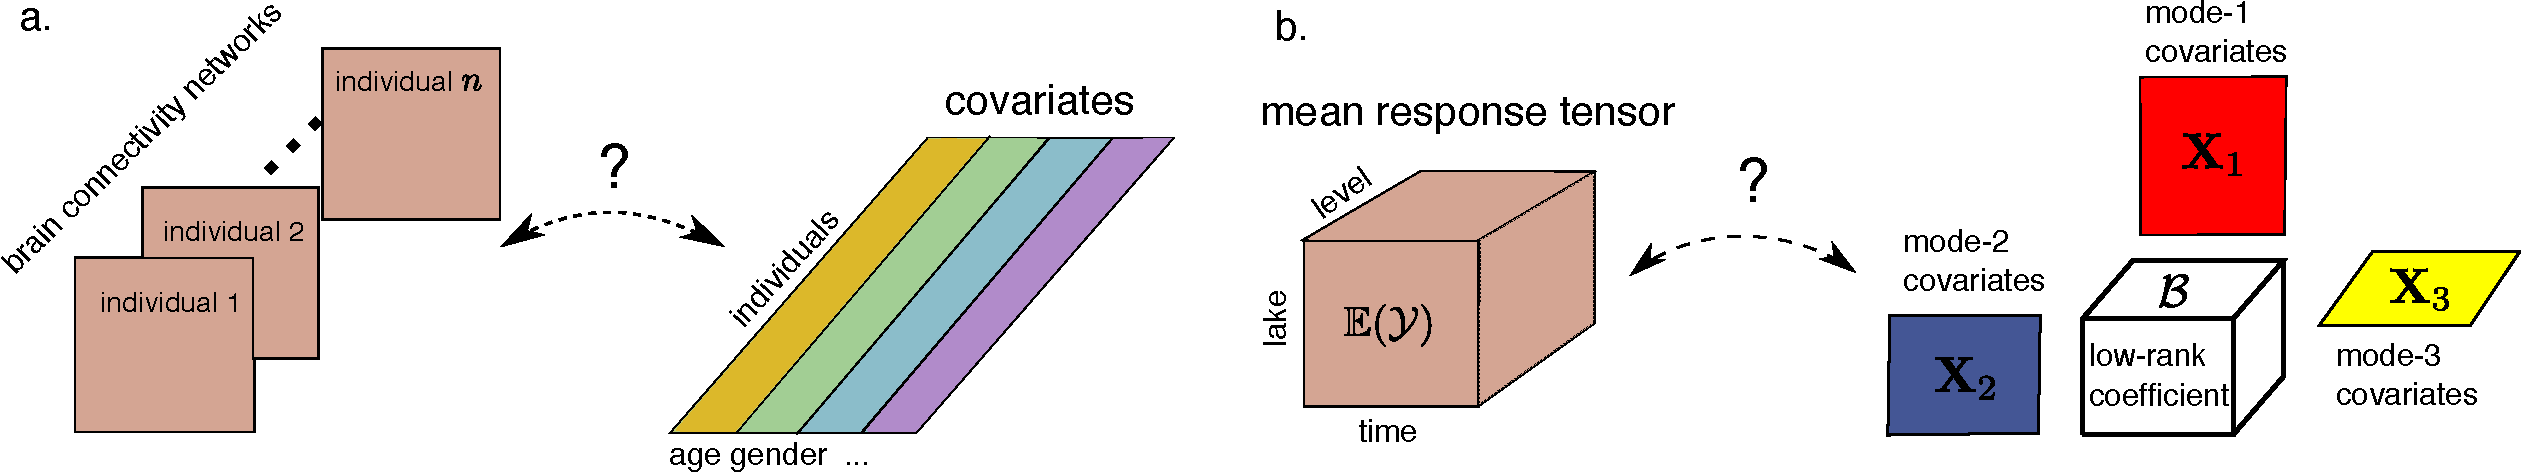
\includegraphics[width=16cm]{demo.pdf}
\end{center}
\caption{Examples of tensor response regression model with covariates on multiple modes. (a) Network population model. (b) Spatial-temporal growth model. }\label{fig:intro1}
\end{figure*}

\vspace{-.1cm}
\section{Preliminaries}
\vspace{-.1cm}
We begin by reviewing the basic properties about tensors~\cite{kolda2009tensor}. We use $\tY=\entry{y_{i_1,\ldots,i_K}}\in \mathbb{R}^{d_1\times \cdots\times d_K}$ to denote an order-$K$ $(d_1,\ldots,d_K)$-dimensional tensor. The multilinear multiplication of a tensor $\tY\in\mathbb{R}^{d_1\times \cdots\times d_K}$ by matrices $\mX_k=\entry{x_{i_k,j_k}^{(k)}}\in\mathbb{R}^{p_k\times d_k}$ is defined as
\begin{equation}
\tY \times_1\mX_1\ldots \times_K \mX_K=\entry{\sum_{i_1,\ldots,i_K}y_{i_1,\ldots,i_K}x_{i_1,j_1}^{(1)}\ldots x_{i_K,j_K}^{(K)}},
\end{equation}
which results in an order-$K$ $(p_1,\ldots,p_K)$-dimensional tensor. For ease of presentation, we use shorthand notion $\tY\times\{\mX_1,\ldots,\mX_K\}$ to denote the tensor-by-matrix product. For any two tensors $\tY=\entry{y_{i_1,\ldots,i_K}}$, $\tY'=\entry{y'_{i_1,\ldots,i_K}}$ of identical order and dimensions, their inner product is defined as $\langle \tY, \tY'\rangle =\sum_{i_1,\ldots,i_K}y_{i_1,\ldots,i_K}y'_{i_1,\ldots,i_K}$. The Frobenius norm of tensor $\tY$ is defined as $\FnormSize{}{\tY}=\langle \tY,\ \tY \rangle^{1/2}$. A higher-order tensor can be reshaped into a lower-order object~\cite{wang2017operator}. We use $\text{vec}(\cdot)$ to denote the operation that reshapes the tensor into a vector, and $\text{Unfold}_k(\cdot)$ the operation that reshapes the tensor along mode-$k$ into a matrix of size $d_k$-by-$\prod_{i\neq k}d_i$. The Tucker rank of an order-$K$ tensor $\tY$ is defined as a length-$K$ vector $\mr=(r_1,\ldots,r_K)$, where $r_k$ is the rank of matrix $\text{Unfold}_k(\tY)$, $k=1,\ldots,K$. We use lower-case letters (e.g.,\ $a,b,c$) for scalars/vectors, upper-case boldface letters (e.g.,\ $\mA,\mB,\mC,$) for matrices, and calligraphy letters (e.g.,\ $\tA, \tB, \tC,$) for tensors of order three or greater. We let $\mI_d$ denote the $d \times d$ identity matrix, $[d]$ denote the $d$-set $\{1,\ldots,d\}$, and allow an $\mathbb{R}\to \mathbb{R}$ function to be applied to tensors in an element-wise manner. 


\section{Motivation and model}\label{sec:model}
Let $\tY=\entry{y_{i_1,\ldots,i_K}}\in\mathbb{R}^{d_1\times \cdots\times d_K}$ denote an order-$K$ data tensor. Suppose we observe covariates on some of the $K$ modes. Let $\mX_k\in\mathbb{R}^{d_k\times p_k}$ denote the available covariates on the mode $k$, where $p_k\leq d_k$. We propose a multilinear structure on the conditional expectation of the tensor. Specifically, 
\begin{align}\label{eq:tensormodel}
&\mathbb{E}(\tY|\mX_1,\ldots,\mX_K)=f(\Theta),\ \text{with}\\
&\Theta =\tB\times\{\mX_1,\ldots,\mX_K\} ,
\end{align}
where $f(\cdot)$ is a known link function, $\Theta\in\mathbb{R}^{d_1\times \cdots\times d_K}$ is the linear predictor, $\tB\in\mathbb{R}^{p_1\times \cdots \times p_K}$ is the parameter tensor of interest, and $\times$ denotes the tensor Tucker product. The choice of link function depends on the distribution of the response data. Some common choices are identity link for Gaussian tensor, logistic link for binary tensor, and $\exp(\cdot)$ link for Poisson tensor (see Table~\ref{table:link}). 

We give three concrete examples of tensor regression that arise in practice. 
\begin{example}[Spatio-temporal growth model]
Let $\tY=\entry{y_{ijk}}\in\mathbb{R}^{d \times m\times n}$ denote the pH measurements of $d$ lakes at $m$ levels of depth and for $n$ time points. Suppose the sampled lakes belong to $q$ types, with $p$ lakes in each type. Let $\{\ell_j\}_{j\in[m]}$ denote the sampled depth levels and $\{t_k\}_{k\in[n]}$ the time points. Assume that the expected pH trend in depth is a polynomial of order $r$ and that the expected trend in time is a polynomial of order $s$. Then, the spatio-temporal growth model can be represented as
\begin{equation}\label{eq:time}
\mathbb{E}(\tY|\mX_1,\mX_2,\mX_3)=\tB\times\{\mX_1,\mX_2,\mX_3\},
\end{equation}
where $\tB\in\mathbb{R}^{p\times (r+1)\times (s+1)}$ is the coefficient tensor of interest, $\mX_1=\text{blockdiag}\{\mathbf{1}_p,\ldots,\mathbf{1}_p\}\in \{0,1\}^{d\times p}$ is the design matrix for lake types, 
\[
\mX_2=
\begin{pmatrix}
1 & \ell_1&\cdots &\ell^{r}_1\\
1 & \ell_2&\cdots &\ell^{r}_2\\
\vdots &\vdots&\ddots&\vdots\\
1&\ell_{m}&\cdots&\ell^{r}_{m}
\end{pmatrix},\
\mX_3=
\begin{pmatrix}
1 & t_1&\cdots &t^{s}_1\\
1 & t_2&\cdots &t^{s}_2\\
\vdots &\vdots&\ddots&\vdots\\
1&t_{n}&\cdots&t^{s}_{n}
\end{pmatrix}
\]
are the design matrices for spatial and temporal effects, respectively. The model~\eqref{eq:time} is a higher-order extension of the ``growth curve'' model originally proposed for matrix data~\cite{gabriel1998generalised,potthoff1964generalized,srivastava2008models}. Clearly, the spatial-temporal model is a special case of our tensor regression model, with covariates available on each of the three modes. 

\end{example}
\begin{example}[Network population model] 
Network response model is recently developed in the context of neuroimanig analysis. The goal is to study the relationship between network-valued response and the individual covariates. Suppose we observe $n$ i.i.d.\ observations $\{(\mY_i, \mx_i): i=1,\ldots,n\}$, where $\mY_i\in\{0,1\}^{d\times d}$ is the brain connectivity network on the $i$-th individual, and $\mx_i\in\mathbb{R}^p$ is the individual covariate such as age, gender, cognition, etc. The network-response model~\cite{rabusseau2016low, zhang2018network} has the form
\begin{equation}\label{eq:network}
\text{logit}(\mathbb{E}(\mY_i|\mx_i))=\tB\times_3\mx_i, \quad \text{for }i=1,\ldots,n
\end{equation}
where $\tB\in \mathbb{R}^{d\times d\times p}$ is the coefficient tensor of interest. 

The model~\eqref{eq:network} is a special case of our tensor-response model, with covariates on the last mode of the tensor. Specifically, stacking $\{\mY_i\}$ together
yields an order-3 response tensor $\tY\in\{0,1\}^{d\times d\times n}$, along with covariate matrix $\mX=[\mx_1,\ldots,\mx_n]\in\mathbb{R}^{p\times n}$. Then, the model~\eqref{eq:network} can be written as
\[
\text{logit}(\mathbb{E}(\tY|\mX))=\tB\times_3 \mX=\tB\times\{\mI_d, \mI_d, \mX\}.
\]
 \end{example}
 
 \begin{example}[Dyadic data with node attributes] Dyadic dataset consists of measurements on pairs of objects or under a pair of conditions. Common examples include networks and graphs. Let $\tG=(V,E)$ denote a network, where $V=[d]$ is the node set of the graph, and $E\subset V\times V$ is the edge set. Suppose that we also observe covariate $\mx_i\in\mathbb{R}^p$ associated to each $i\in V$. A probabilistic model on the graph $\tG=(V,E)$ can be described by the following matrix regression. The edge connects the two vertices $i$ and $j$ independently of other pairs, and the probability of connection is modeled as
\begin{equation}\label{eq:edge}
 \text{logit}(\mathbb{P}((i,j)\in E)=\mx^T_i\mB\mx_j=\langle \mB, \mx^T_i\mx_j\rangle.
 \end{equation}
The above model has demonstrated its success in modeling transitivity, balance, and communities in the networks~\cite{hoff2005bilinear}. We show that our tensor regression model~\eqref{eq:tensormodel} also incorporates the graph model as a special case. Let $\tY=\entry{y_{ij}}$ be a binary matrix where $y_{ij}=\mathds{1}_{(i,j)\in E}$. Define $\mX=[\mx_1,\ldots,\mx_n]\in\mathbb{R}^{p\times n}$. Then, the graph model~\eqref{eq:edge} can be expressed as
 \[
 \text{logit}(\mathbb{E}(\mY|\mX))=\tB\times\{\mX,\mX\}.
 \]
\end{example}

In the above three examples and many other studies, researchers are interested in uncovering the variation in the data tensor that can be explained by the covariates. The regression coefficient $\tB$ in our model model~\eqref{eq:tensormodel} serves this goal by collecting the effects of covariates and the interaction thereof.  
To encourage the sharing among effects, we assume that the coefficient tensor $\tB$ lies in a low-dimensional parameter space:
\begin{equation}\label{eq:rank}
\small \tP_{r_1,\ldots,r_K}=\{\tB\in\mathbb{R}^{p_1\times \cdots \times p_K}: r_k(\tB)\leq r_k \text{ for all } k\in[K]\},
\end{equation}
where $r_k(\tB)\leq p_k$ is the Tucker rank at mode $k$ of the tensor. The low-rank assumption is plausible in many scientific applications. In brain imaging analysis, for instance, it is often believed that the brain nodes can be grouped into fewer communities, and the numbers of communities are much smaller than the number of nodes. The low-rank structure encourages the shared information across tensor entries, thereby greatly improving the estimation stability. When no confusion arises, we drop the subscript $(r_1,\ldots,r_K)$ and write $\tP$ for simplicity.


Our tensor regression model is able to incorporate covariates on any subset of modes, whenever available. Without loss of generality, we denote by $\tX=\{\mX_1,\ldots,\mX_K\}$ the covariates in all modes and treat $\mX_k=\mI_{d_k}$ if the mode-$k$ has no (informative) covariate. Then, the final form of our tensor regression model can be written as:
\begin{align}\label{eq:tensormodel}
&\mathbb{E}(\tY|\tX)=f(\Theta),\quad \Theta =\tB\times\{\mX_1,\ldots,\mX_K\},\notag\\
&\text{where}\ \text{rank}(\tB)\leq (r_1,\ldots,r_K),
\end{align}
where the entries of $\tY$ are independent r.v.'s conditional on $\tX$, and $\tB\in\mathbb{R}^{p_1\times \cdots\times p_K}$ is the low-rank coefficient tensor of interest. We comment that other forms of tensor low-rankness are also possible, and here we choose Tucker rank just for parsimony. Similar models can be derived using various notions of low-rankness based on CP decomposition~\cite{hitchcock1927expression} and train decomposition~\cite{oseledets2011tensor}. 

\section{Rank-constrained likelihood-based estimation}
We develop a likelihood-based procedure to estimate the coefficient tensor $\tB$ in~\eqref{eq:tensormodel}. We adopt the exponential family as a flexible framework for different data types. In a classical generalized linear model (GLM) with a scalar response $y$ and covariate $\mx$, the density is expressed as:
\[
p(y|\mx, \boldsymbol{\beta})=c(y)\exp\left({y\theta- b(\theta) \over \phi}\right)\ \text{with}\ \theta=\boldsymbol{\beta}^T\mx,
\]
where $b(\cdot)$ is a known function, $\theta$ is the linear predictor, $\phi>0$ is the dispersion parameter, and $c(\cdot)$ is a known normalizing function. The choice of link functions depends on the data types and on the observation domain of $y$, denoted $\mathbb{Y}$. For example, the observation domain is $\mathbb{Y}=\mathbb{R}$ for continuous data, $\mathbb{Y}=\mathbb{N}$ for count data, and  $\mathbb{Y}=\{0,1\}$ for binary data. 
Note that the canonical link function $f$ is chosen to be $f(\cdot)=b'(\cdot)$. Table~1 summarizes the canonical link functions for common types of distributions. 

\begin{table}
\centering
\begin{tabular}{c|ccc}
Data type &Gaussian & Poisson& Bernoulli\\
\hline
Domain $\mathbb{Y}$& $\mathbb{R}$&$\mathbb{N}$&$\{0,1\}$\\
 $b(\theta)$&$\theta^2/2$& $\exp(\theta)$&$\log (1+\exp(\theta))$\\
 link $f(\theta)$&$\theta$&$\exp(\theta)$&$(1+\exp(-\theta))^{-1}$
\end{tabular}
\caption{Canonical links for common distributions.}\label{table:link}
\end{table}

In our context, we model the the entries in the response tensor $y_{ijk}$ conditional on $\theta_{ijk}$ as independent draws from an exponential family. The quasi log-likelihood of~\eqref{eq:tensormodel} is equal (ignoring constant) to Bregman distance between $\tY$ and $b'(\Theta)$:
\begin{align}
\tL_{\tY}(\tB)&=\langle \tY, \Theta \rangle - \sum_{i_1,\ldots,i_K} b(\theta_{i_1,\ldots,i_K}),\\
\text{where}\ \Theta&=\tB\times\{\mX_1,\ldots,\mX_K\}.
\end{align}
We assume that we have an additional information on an upper bound $\alpha>0$ such that $\mnormSize{}{\Theta}\leq \alpha$. This is the case for many applications we have in mind such as brain network analysis where fiber connections are bounded. We propose a constrained maximum likelihood estimator (MLE) for the coefficient tensor:
\begin{equation}\label{eq:MLE}
\hat \tB=\argmax_{\text{rank}(\tB)= \mr, \mnormSize{}{\Theta(\tB)}\leq \alpha} \tL_{\tY}(\tB).
\end{equation}
In the following theoretical analysis, we assume the rank $\mr=(r_1,\ldots,r_K)$ is known and fixed. The adaptation of unknown $\mr$ will be addressed in Section~\ref{sec:tuning}. 


\subsection{Statistical properties}
We assess the estimation accuracy using the deviation in the Frobenius norm. For the true coefficient tensor $\trueB$ and its estimator $\hat \tB$, define
\[
\text{Loss}(\trueB,\ \hat \tB)=\FnormSize{}{\trueB- \hat \tB}^2.
\]

In modern applications, the response tensor and covariates are often large-scale. We are particularly interested in the high-dimensional region in which both $d_k$ and $p_k$ diverge; i.e.\ $d_k\to \infty$ and $p_k\to\infty$, while ${p_k\over d_k} \to \gamma_k \in[0,1)$. As the size of problem grows, and so does the number of unknown parameters. As such, the classical MLE theory does not directly apply. We leverage the recent development in random tensor theory and high-dimensional statistics to establish the error bounds of the estimation. 

  
  
\begin{assumption}\label{ass}We make the following assumptions:
\begin{enumerate}
\item [A1.] There exist two positive constants $c_1, c_2>0$ such that $c_1\leq \sigma_{\min}(\mX_k)\leq  \sigma_{\max}(\mX_k)\leq c_2$ for all $k\in[K]$. Here $\sigma_{\text{min}}(\cdot)$ and $\sigma_{\text{max}}(\cdot)$ denotes the smallest and largest singular values, respectively.
\item [A2.] There exist two positive constants $L,\ U>0$ such that $L\leq \text{Var}(y_{i_1,\ldots,i_K}|\theta_{i_1,\ldots,i_K})\leq U$ for all $|\theta_{i_1,\ldots,i_K}|\leq \alpha$.
\item[A2'.] Equivalently, there exists two positive constants $L,\ U>0$ such that $L\leq b''(\theta) \leq U$ for all $|\theta|\leq \alpha$, where $\alpha$ is the upper bound of the linear predictor. 

\end{enumerate}
\end{assumption}
The assumptions are fairly mild. Assumption A1 guarantees the non-singularity of the covariates, and Assumption A2 ensures the log-likelihood $\tY(\Theta)$ is strictly concave in the linear predictor $\Theta$. Assumption A2 and A2' are equivalent, because $\text{Var}(y_{i_1,\ldots,i_K}|\tX,\tB)=b''(\theta_{i_1,\ldots,i_K})$ when $y_{i_1,\ldots,i_K}$ belongs to an exponential family~\cite{mccullagh1989generalized}. 

  
\begin{thm}[Statistical convergence]\label{thm:main}
Consider a generalized tensor regression model with covariates on multiple modes $\tX=\{\mX_1,\ldots,\mX_K\}$. Suppose the entries in $\tY$ are independent realizations of an exponential family distribution, and $\mathbb{E}(\tY|\tX)$ follows the low-rank tensor regression model~\eqref{eq:tensormodel}. Under Assumption~\ref{ass}, there exist two constants $C_1, C_2>0$, such that, with probability at least $1-\exp(-C_1\sum_k p_k)$, 
\begin{equation}\label{eq:bound}
\text{Loss}(\trueB,\ \hat \tB) \leq C_2\sum_k p_k.
\end{equation}
Here, $C_2=C_2(\mr,\alpha, K)>0$ is a constant that does not depend on the dimensions $\{d_k\}$ and $\{p_k\}$. 
\end{thm}

To gain further insight on the bound~\eqref{eq:bound}, we consider a special case when tensor dimensions are equal at each of the modes, i.e., $d_k=d$, $p_k=\gamma d$, $\gamma\in [0,1)$ for all $k\in[K]$, and the covariates $\mX_k$ are Gaussian design matrices with i.i.d.\ $N(0,\sigma^2)$ entries. To put the context in the framework of Theorem~\ref{thm:main}, we rescale the covariates into $\check \mX_k={1\over \sqrt{d}}\mX_k$ so that the singular values of $\check \mX_k$ are bounded by $1\pm \sqrt{\gamma}$. The result in~\eqref{eq:bound} implies that the estimated coefficient has a convergence rate $\tO({p\over d^K})$ in the scale of the original covariates $\{\mX_k\}$. Therefore, our estimation is consistent as the dimension grows, and the convergence becomes especially favorably as the order of tensor data increases. 

As immediate applications, we obtain the convergence rate for the three examples mentioned in Section~\ref{sec:model}. Without loss of generality, we assume that the singular values of the $d_k$-by-$p_k$ covariate matrix $\mX_k$ are bounded by $\sqrt{d_k}$. 


\begin{cor}[Spatio-temporal growth model] The estimated type-by-time-by-space coefficient tensor converges at the rate $\tO\left({p+r+s\over dmn}\right)$ where $p\leq d$, $r\leq m$ and $s\leq n$. The estimation achieves consistency as long as the dimension grows in either of the three modes.
\end{cor}

\begin{cor} [Network population model] The estimated node-by-node-by-covariate tensor converges at the rate $\tO\left({2d+p\over d^2n}\right)$ where $p\leq n$. The estimation achieves consistency as the number of individuals or the number of nodes grows. 
\end{cor}

\begin{cor} [Dyadic data with node attributes] The estimated covariate-by-covariate matrix converges at the rate $\tO\left({p\over d^2}\right)$ where $p\leq d$. Again, our estimation achieves consistency as the number of nodes grows. 
\end{cor}

We conclude this section by providing the prediction accuracy, measured in KL divergence, for the response distribution.   

\begin{thm}[Prediction error]\label{thm:KL}
Assume the same set-up as in Theorem~\ref{thm:main}. Let $\mathbb{P}_{\tY_{\text{true}}}$ and $\mathbb{P}_{\hat \tY}$ denote the distributions of $\tY$ given the true parameter $\trueB$ and estimated parameter $\hat \tB$, respectively. Then, we have, with probability at least $1-\exp(C_1\sum_k p_k)$,
\[
\text{KL}(\mathbb{P}_{\tY_{\text{true}}},\ \mathbb{P}_{\hat \tY})\leq C_4 \sum_k p_k,
\]
where $C_4=C_4(\mr,\alpha, K)>0$ is a constant that do not depend on the dimensions $\{d_k\}$ and $\{p_k\}$.
\end{thm}


\section{Numerical implementation}
\subsection{Alternating optimization}
In this section, we introduce an efficient algorithm to solve~\eqref{eq:MLE}. The objective function $\tL_{\tY}(\tB)$ is concave in $\tB$ when the link $f$ is the canonical link function. However, the feasible set $\tP$ is non-convex, and thus the optimization~\eqref{eq:MLE} is a non-convex problem. We utilize a Tucker factor representation of the coefficient tensor $\tB$ and turn the optimization into a block-wise convex problem. 

Specifically, write the rank-$\mr$ decomposition of coefficient tensor $\tB$ as
\begin{equation}\label{eq:tucker}
\tB=\tC\times \{\mM_1,\ldots,\mM_K\},
\end{equation}
where $\tC\in\mathbb{R}^{r_1\times\cdots\times r_K}$ is a full-rank core tensor, $\mM_k\in\mathbb{R}^{p_k\times r_k}$ are factor matrices with orthogonal columns. Estimating $\tB$ amounts to finding both the core tensor $\tC$ and the factor matrices $\mM_k$'s. The optimization~\eqref{eq:MLE} can be written as $(\hat \tC, \{\hat \mM_k\})=\arg\max \tL_{\tY}(\tC, \mM_1,\ldots,\mM_K)$, where
\begin{align}
\tL_{\tY}(\tC, \mM_1,\ldots,\mM_K )&=\langle \tY, \Theta\rangle -\sum_{i_1,\ldots,i_K}b(\theta_{i_1,\ldots,i_K}),\\
\text{with } \Theta&=\tC\times\{\mM_1\mX_1,\ldots,\mM_K\mX_K\}.
\end{align}
The decision variables in the above objective function consist of $K+1$ blocks of variables, one for the core tensor $\tC$ and $K$ for the factor matrices $\mM_k$'s. We notice that, if any $K$ out of the $K+1$ blocks of variables are known, then the optimization with respect to the last block of variables reduced to a simple GLM. This observation suggests that we can iteratively update one block at a time while keeping others fixed. 

Suppose the core tensor $\tC$ and the factor matrix $\mM_k$ are known for $k=1,\ldots,K-1$. It turns out that last factor matrix $\mM_K$ can be solved in a row-by-row fashion via $p_k$ separate GLMs. To see this, let $\tC^{(t)}$ denote the core tensor at the $t$-th iteration,  $\mM^{(t)}_k$ the $k$th factor matrix for $k\in[K-1]$, and define
\[
\mX^{(t)}_{-K}=\tC^{(t)}\times \{ \mM^{(t)}_1\mX_1,\ \ldots,\ \mM^{(t)}_{K-1}\mX_{K-1}\},
\]
Then, the objective function implies that the $i$-th row of $\mM^{(t)}_K$ is the ``regression coefficient'' for a GLM whose response is a vector $\text{vec}(\tY(:,\ :, \ i))\in\mathbb{R}^{d_{-K}}$ and covariate matrix is $\text{Unfold}_K(\mX_{-K}^{(t)})\in\mathbb{R}^{d_{-K} \times r_K}$, with $d_{-K}\stackrel{\text{def}}{=}\prod_{k\in[K-1]}d_k$. This property of seperation by row allows us to leverage state-of-art GLM solvers and parallel processing to achieve computational efficiency. 

After each iteration, we rescale the core tensor $\tC^{(t+1)}$ subject to the infinity norm constraint. This post-processing in principle may not guarantee the monotonic increase of the objective, but we found that in our experiment this simple step appears robust for obtaining a desirable solution. The full algorithm is described in Algorithm~1.

\begin{figure*}[t]
\begin{center}
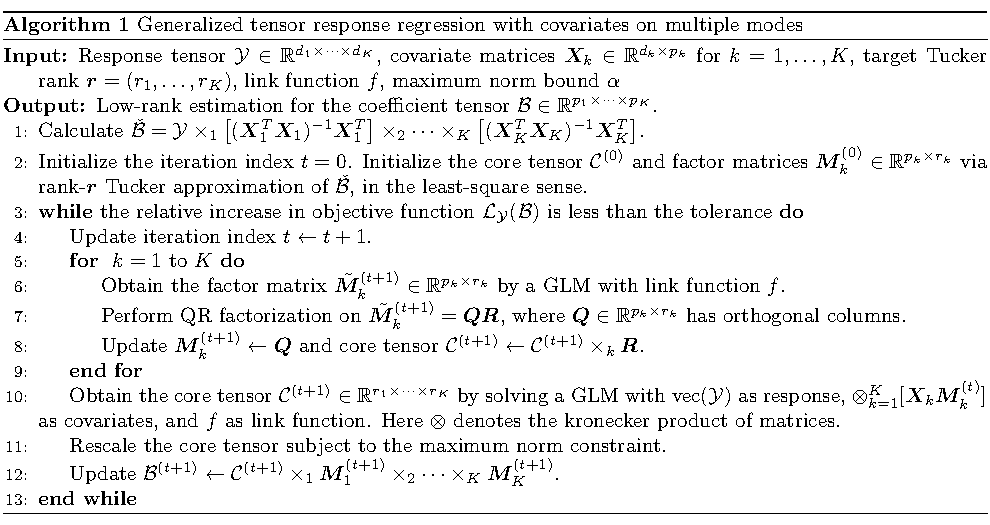
\includegraphics[width=17.5cm]{algorithm.pdf}
  \end{center}
  \end{figure*}

\subsection{Rank selection}\label{sec:tuning}
Algorithm~1 takes the rank $\mr$ as an input. Estimating an appropriate rank given the data is of practical importance. We propose to use Bayesian information criterion (BIC) and choose the rank that minimizes BIC; i.e.
\begin{align}\label{eq:BIC}
\hat \mr&=\argmin_{\mr=(r_1,\ldots,r_K)} \text{BIC}(\mr)\\
&=\argmin_{\mr=(r_1,\ldots,r_K)}\left[-2\tL_{\tY}(\hat \tB)+p_e(\mr)\log \left(\prod_k d_k\right) \right],
\end{align}
where $p_e(\mr)\stackrel{\text{def}}{=}\sum_k (p_k-r_k-1)r_k+\prod_k r_k$ is the effective number of parameters in the model. We choose $\hat \mr$ that minimizes $\text{BIC}(\mr)$ via grid search. Our choice of BIC aims to balance between the goodness-of-fit for the data and the degree of freedom in the population model. We test its empirical performance in Section~\ref{sec:simulation}.  

\section{Simulation}\label{sec:simulation}
We evaluate the empirical performance of our generalized tensor regression through simulations. We consider order-3 tensors with a range of distribution types. The coefficient tensor $\tB$ is generated using the factorization form~\eqref{eq:tucker} where both the core and factor matrices are drawn i.i.d.\ from Uniform[0,1]. The linear predictor is then simulated from $\tU=\tB\times\{\mX_1,\mX_2,\mX_3\}$, where $\mX_k$ is either an identity matrix (i.e.\ no covariate available) or Gaussian random matrix with i.i.d.\ entries from $N(0,\sigma^2)$. We set $\sigma^2=d_k^{-1/2}$ to ensure the singular values of $\mX_k$ are bounded as $d_k$ increases. The $\tU$ is scaled such that $\mnormSize{}{\tU}=1$. Conditional on the linear predictor $\tU=\entry{u_{ijk}}$, the entries in the tensor $\tY=\entry{y_{ijk}}$ are drawn independently according to one of the following three probabilistic models:

\begin{enumerate}[itemsep=0pt,topsep=0pt]
\item[(a)] (Gaussian). Continuous data $y_{ijk}\sim N\left(\alpha u_{ijk}, 1\right)$.
\item[(b)] (Poisson). Count data $y_{ijk}\sim\text{Poi}\left( e^{\alpha u_{ijk}}\right)$.
\item[(c)] (Bernoulli). Binary data $y_{ijk}\sim \text{Ber}\left( {e^{\alpha u_{ijk}} \over 1+e^{\alpha u_{ijk}}}\right)$.
\end{enumerate}
Here $\alpha>0$ is a scalar controlling the magnitude of the effect size. In each simulation study, we report the mean squared error (MSE) for the coefficient tensor averaged across $n_{\text{sim}}=30$ replications. 

The first experiment assesses the selection accuracy of our BIC criterion~\eqref{eq:BIC}. We consider the balanced situation where $d_k=d$, $p_k=0.4d_k$ for $k=1,2,3$. We set $\alpha=10$, $\alpha=4$, and consider various combinations of dimension $d$ and rank $\mr=(r_1,r_2,r_3)$. For each combination, we simulate tensor data following Gaussian, Bernoulli, and Poisson models. We then minimize BIC using a grid search over three dimensions. The hyper-parameter $\alpha$ is set to infinity in the fitting, which essentially imposes no prior on the coefficient magnitude. Table~\ref{tab:rank} reports the selected rank averaged over $n_{\text{sim}}=30$ replicates for Gaussian and Poisson models. We found that when $d=20$, the selected rank is slightly smaller than the true rank, and the accuracy improves immediately when the dimension increases to $d=40$. This agrees with our expectation, as in tensor regression, the sample size is related to the number of entries. A larger $d$ implies a larger sample size, so the BIC selection becomes more accurate. 


\begin{table}[t]
\centering
%\resizebox{1\textwidth}{!}{
\begin{tabular}{|c|cc|cc|}
\hline
True Rank &\multicolumn{2}{c|}{Dimension (Gaussian tensors)}&\multicolumn{2}{c|}{Dimension (Poisson tensors)}\\
$\mr$& $d=20$  &$d=40$&$d=20$ &$d=40$\\
\hline
$(3,\ 3,\ 3)$&$(2.1,\ 2.0,\ 2.0)$&$({\bf 3},\ {\bf 3},\ {\bf 3})$&$(2.0,\ 2.2,\ 2.1)$&$({\bf 3},\ {\bf 3},\ {\bf 3})$\\
$(4,\ 4,\ 6)$&$(3.2,\ 3.1,\ 5.0)$&$({\bf 4},\ {\bf 4},\ {\bf 6})$&$({\bf 4.0},\ {\bf 4.0},\ 5.2)$&$({\bf 4},\ {\bf 4},\ {\bf 6})$\\
$(6,\ 8,\ 8)$&$(5.1,\ 7.0,\ 6.9)$&$({\bf 6},\ {\bf 8},\ {\bf 8})$&$(5.0,\ 6.1,\ 7.1)$&$({\bf 6},\ {\bf 8},\ {\bf 8})$\\
\hline
\end{tabular}
%}
\caption{Rank selection via BIC. Bold number indicates no significant difference between the estimate and the ground truth, based on a $z$-test with a level 0.05.}\label{tab:rank}
\end{table}

The second experiment evaluates the accuracy when covariates are available on all modes. We set $\alpha=10, d_k=d, r_k=r\in\{2,4,6\}$ and increase $d$ from 25 to 50. Our theoretical analysis suggests that $\hat \tB$ has a convergence rate $\tO(d^{-2})$ in this setting. Figure~1 plots the estimation error versus the ``effective sample size'', $d^2$, under three different distribution models. We found that the empirical MSE decreases roughly at the rate of $1/d^2$, which is consistent with our theoretical ascertainment. We also observed that, tensors with higher ranks tend to yield higher estimation errors, as reflected by the upward shift of the curves as $r$ increases. Indeed, a larger $r$ implies a higher model complexity and thus greater difficulty in the estimation. Similar behaviors can be observed in the non-Gaussian data in Figure~\ref{fig:dim}b-c. 

\begin{figure}[t]
\centering
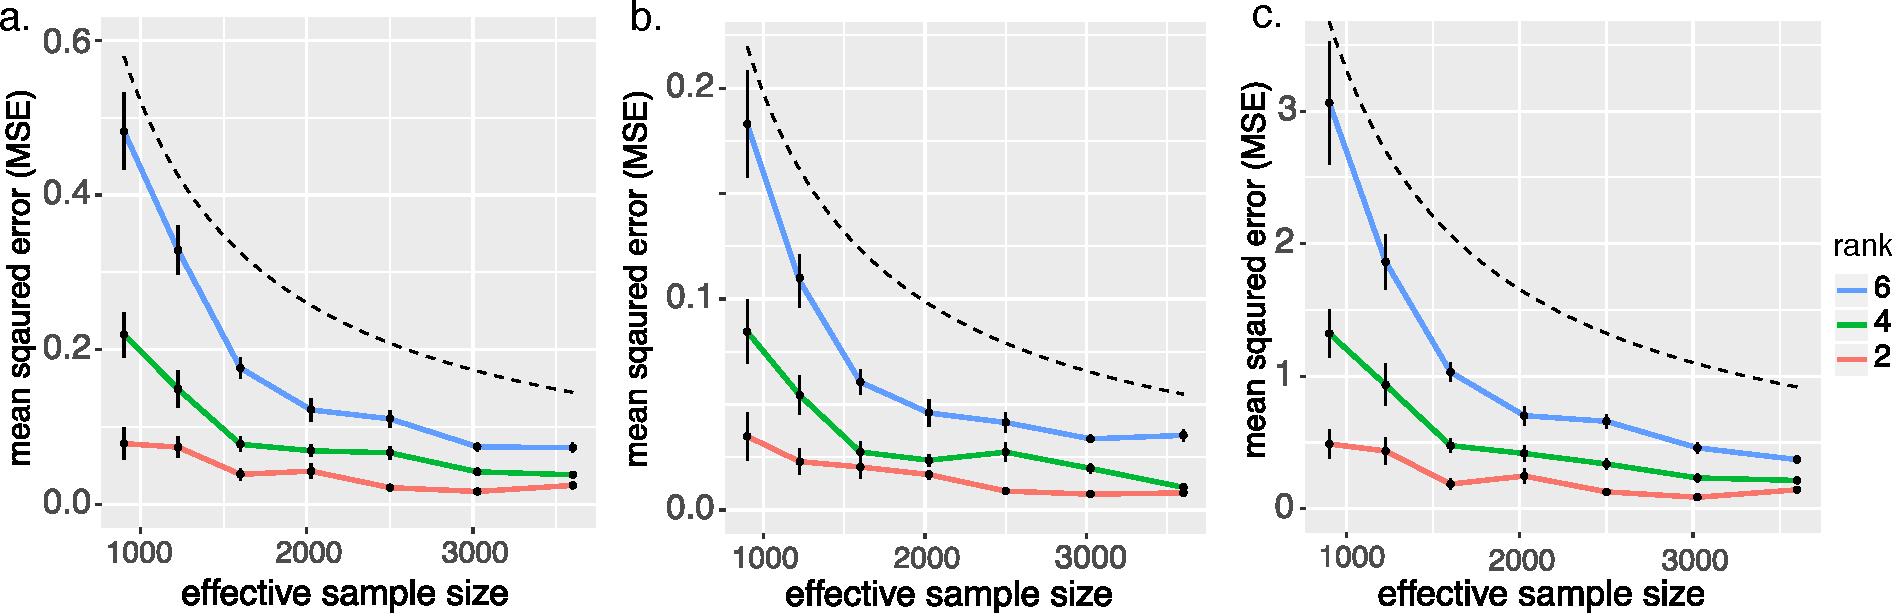
\includegraphics[width=15cm]{dimension.pdf}
\caption{Estimation error against effective sample size. The three panels depict the MSE when the response tensors are generated form (a) Gaussian (b) Poisson and (c) Bernoulli models. The dashed curves correspond to $\tO({1/d^2})$.}\label{fig:dim}
\end{figure}

The third experiment investigates our model's ability in handling correlation among coefficients. We mimic the scenario of brain imaging analysis. A sample of $d_3=50$ networks are simulated, one for each individual. Each network measures the connections between $d_1=d_2=20$ brain nodes. We simulate $p=5$ covariates for the each of the 50 individuals. These covariates may represent, for example, age, gender, cognitive score, etc. Recent study~\cite{robinson2015dynamic} has suggested that brain connectivity networks often exhibit community structure represented as a collection of subnetworks, and each subnetwork is comprised of a set of spatially distributed brain nodes. To accommodate this structure, we utilize the stochastic block model~\cite{abbe2017community} to generate the effect size. Specifically, we partition the nodes into $r$ blocks by assigning each node to a block with uniform probability. Edges within a same block are assumed to share the same covariate effects, where the effects are drawn i.i.d.\ from $N(0,1)$. We then apply our tensor regression model to the network data using the BIC-selected rank. Note that in this case, the true model rank is unknown; the rank of a $r$-block matrix is not necessarily equal to~$r$~\cite{zeng2019multiway}. 



\begin{figure}[t]
\centering
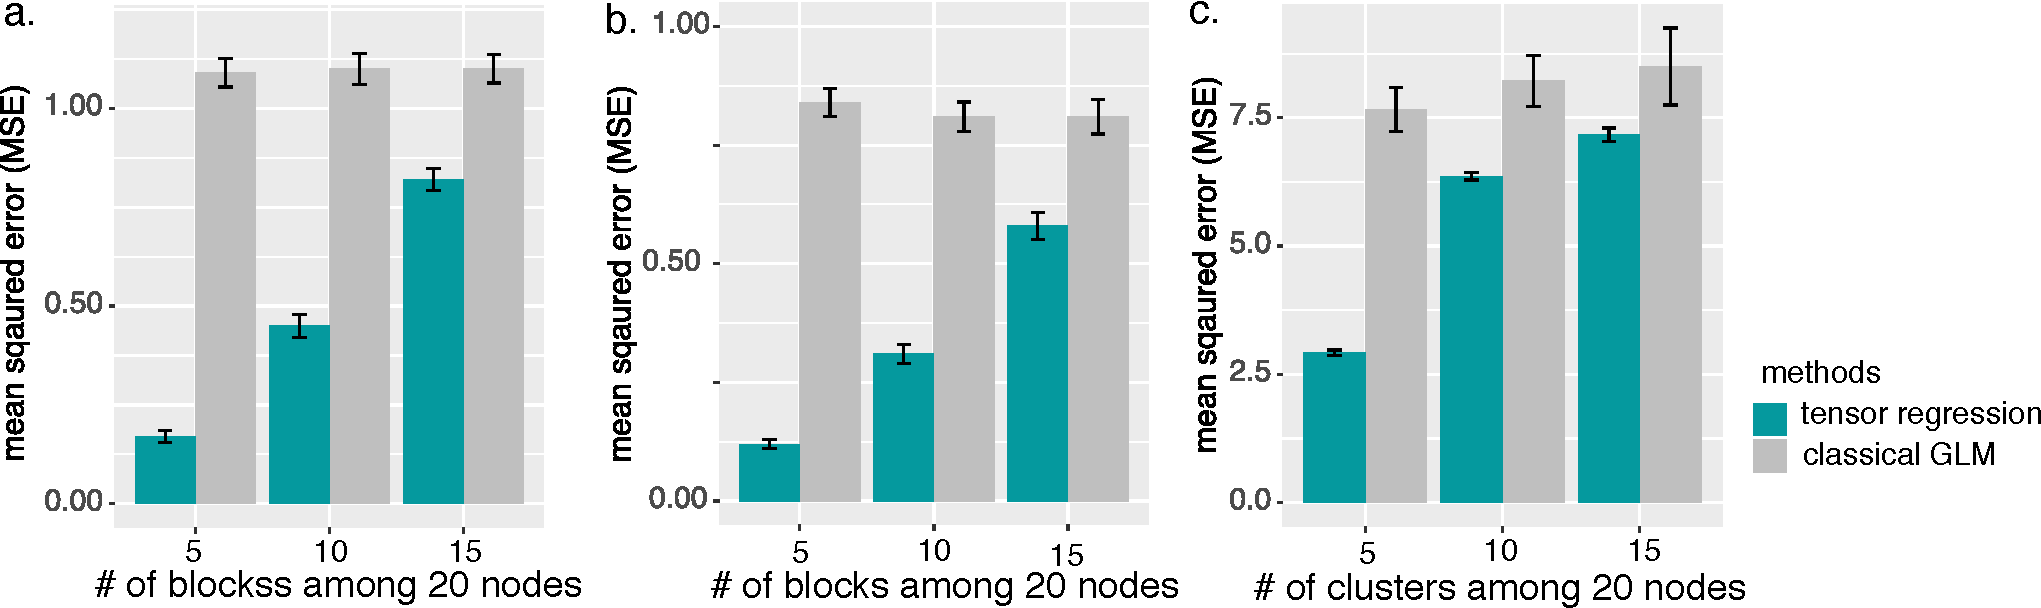
\includegraphics[width=15cm]{comparison.pdf}
\caption{Performance comparison when the networks have block structure. The three panels depict the MSE when the response tensors are generated form (a) Gaussian (b) Poisson and (c) Bernoulli models. The $x$-axis represents the number of blocks in the networks. }\label{fig:glm}
\end{figure}


Figure~\ref{fig:glm} compares the MSE of our method with a classical GLM approach. A classical GLM is to regress the dyadic edges, one at a time, on the covariates, and this model is repeatedly fitted for each edge. This repeated approach, however, does not account for the correlation among the edges, and may suffer from overfitting. As we can see in Figure~\ref{fig:glm}, out tensor regression method achieves significant error reduction in all three models considered. The outer-performance is significant in the presence of large communities, and even in the less structured case ($\sim 20/15=1.33$ nodes per block), our method still outer-performs GLM. This is because the low-rankness in our modeling automatically identifies the shared information across entries. By selecting the rank in a data-driven way, our method is able to achieve accurate estimation with improved interpretability. 




\section{Data analysis}
We apply our tensor regression model to two real datasets. The first application concerns the brain network modeling in response to individual attributes (i.e.\ covariate on one mode), and the second application focuses on multi-relational network analysis with dyadic attributes (i.e.\ covariates on two modes). 
\subsection{Human Connectome Project (HCP)}
The Human connectome project (HCP~\cite{HCP}) aims to build a ``network map'' that characterizes the anatomical and functional connectivity within healthy human brains. We take a subset of HCP data that consists of 136 brain structural networks, one for each individual. Each brain network is represented as a 68-by-68 binary matrix, where the entries encode the presence or absence of fiber connections between the 68 brain regions. We consider four individual-covariates: gender (65 females vs.\ 71 males), age 22-25 ($n=35$), age 26-30 ($n=58$), and age 31+ ($n=43$). The goal is to identify the connection edges that are affected by the individual covariates. A key challenge in brain network is that the edges are correlated; for example, two edges may stem out from a same brain region, and it is of importance to take into account the within-dyad dependence. 


\begin{figure}[t]
\centering
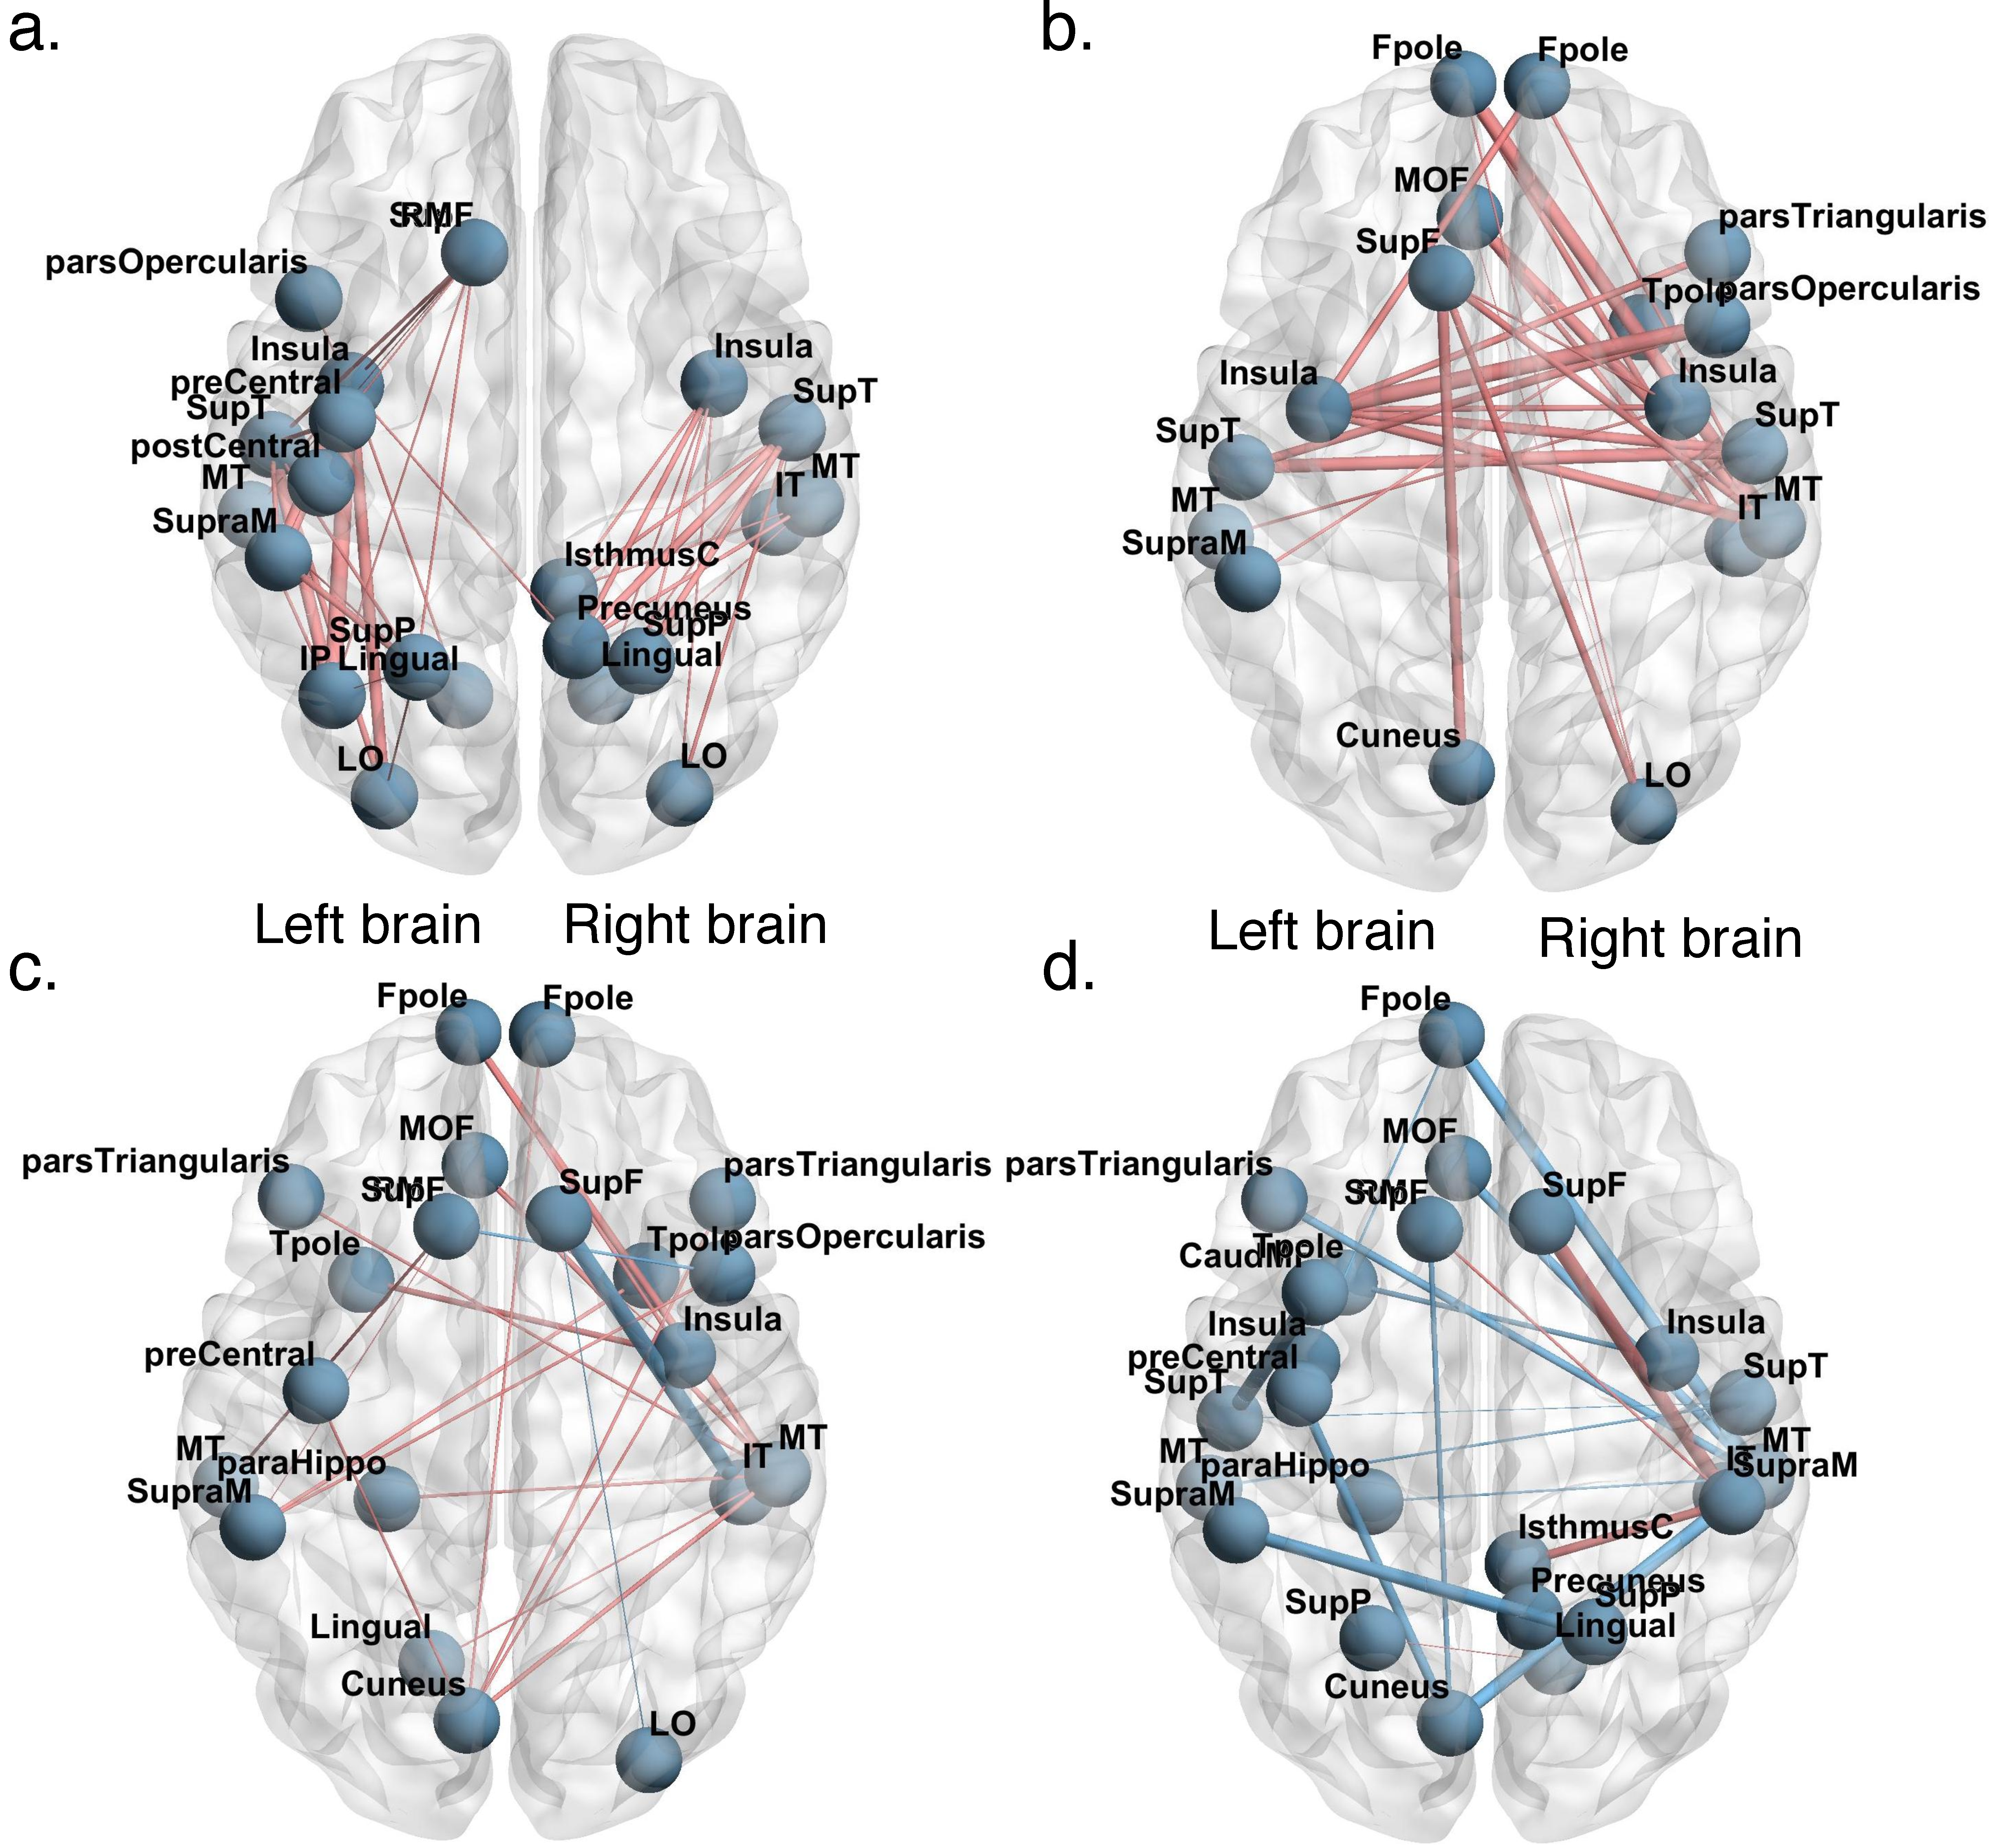
\includegraphics[width=8cm]{HCP.pdf}
\caption{Top edges with large effects. Red edges represent relatively strong connections and blue edges represent relatively weak connections. (a) Global effect; (b) Female effect; (c) Age 22-25; (d) Age 31+.}\label{fig:brain}
\end{figure}

We fit the tensor regression model to the HCP data. The response is a binary tensor $\tY\in\{0,1\}^{68\times 68\times 136}$ and the covariates are of dimension 4 along the 3$^{\text{rd}}$ mode. The BIC selection suggests a rank $\mr=(10,10,4)$ with log-likelihood $\tL_{\tY}=-174654.7$. Figure~\ref{fig:brain} shows the top edges with high effect size, overlaid on the Desikan atlas brain template~\cite{desikan2006automated,xia2013brainnet}. We utilize the sum-to-zero contrasts in the effects coding and depicted only the top 3\% edges whose connections are non-constant across the sample. It is observed that the global connection exhibits clear spatial separation, and that the nodes within each hemisphere are more densely connected with each other (Figure~\ref{fig:brain}a). In particular, the superior-temproal (\emph{SupT}), middle-temporal (\emph{MT}) and Insula are the top three popular nodes in the network. Interestingly, female brains display higher inter-hemispheric connectivity, especially in the frontal, parental and temporal lobes (Figure~\ref{fig:brain}b). This is in agreement with a recent study showing that female brains are optimized for inter-hemispheric communication~\cite{ingalhalikar2014sex}. We also found several edges with declined connection in the group Age 31+. Notably, those edges involve Frontal-pole (\emph{Fploe}), superior-frontal (\emph{SupF}) and Cuneus nodes. The Frontal-pole region has long been known for its importance in memory and cognition, and the detected decline with age further highlights its biological importance. 

\subsection{Nations data}

The second application concerns the multi-relational network analysis with node-level attributes. We consider \emph{Nations} dataset~\cite{nickel2011three} which records 56 relations among 14 countries between 1950 and 1965. The multi-relational networks can be organized into a $14 \times 14 \times 56$ binary tensor, with each entry indicating the presence or absence of a connection, such as ``sending tourist to'', ``export'', ``import'', between countries. The 56 relations span the fields of politics, economics, military, religion, and so on. In addition, country-level attributes are also available, and we focus on the following six covariates: \emph{constitutional, catholics, lawngos, politicalleadership, geographyx}, and \emph{medicinengo}. The goal is to identify the variation in connections due to country-level attributes and interactions thereof. One of the key features is that the 56 relations are correlated, and we would like to take that into account in assessing the covariate effects. 

We applied our tensor regression model to the \emph{Nations} data. The multi-relational network $\tY\in\{0,1\}^{14\times 14\times 56}$ was treated as the response tensor, and the country attributes $\mM\in\mathbb{R}^{14\times 6}$ were treated as covariates on both the 1st and 2nd modes. The BIC criterion suggests a rank $\mr=(4,4,4)$ for the coefficient tensor $\tB\in\mathbb{R}^{6\times 6 \times 56}$. Supplementary Table S1 shows the $K$-mean clustering of the 56 relations based on the 3$^\text{rd}$ mode factor $\mM_3\in\mathbb{R}^{56\times 4}$. We found that the relations reflecting the similar aspects of international affairs are grouped together. In particular, Cluster I consists of political relations such as \emph{officialvisits, intergovorgs}, and \emph{militaryactions}; Clusters II and III capture the economical relations such as \emph{economicaid, booktranslations, tourism}; and Cluster IV represents the Cold War alliance blocs. The similarity among entities in each cluster suggests the plausibility of our dimension reduction. 

\begin{figure}[t]
\centering
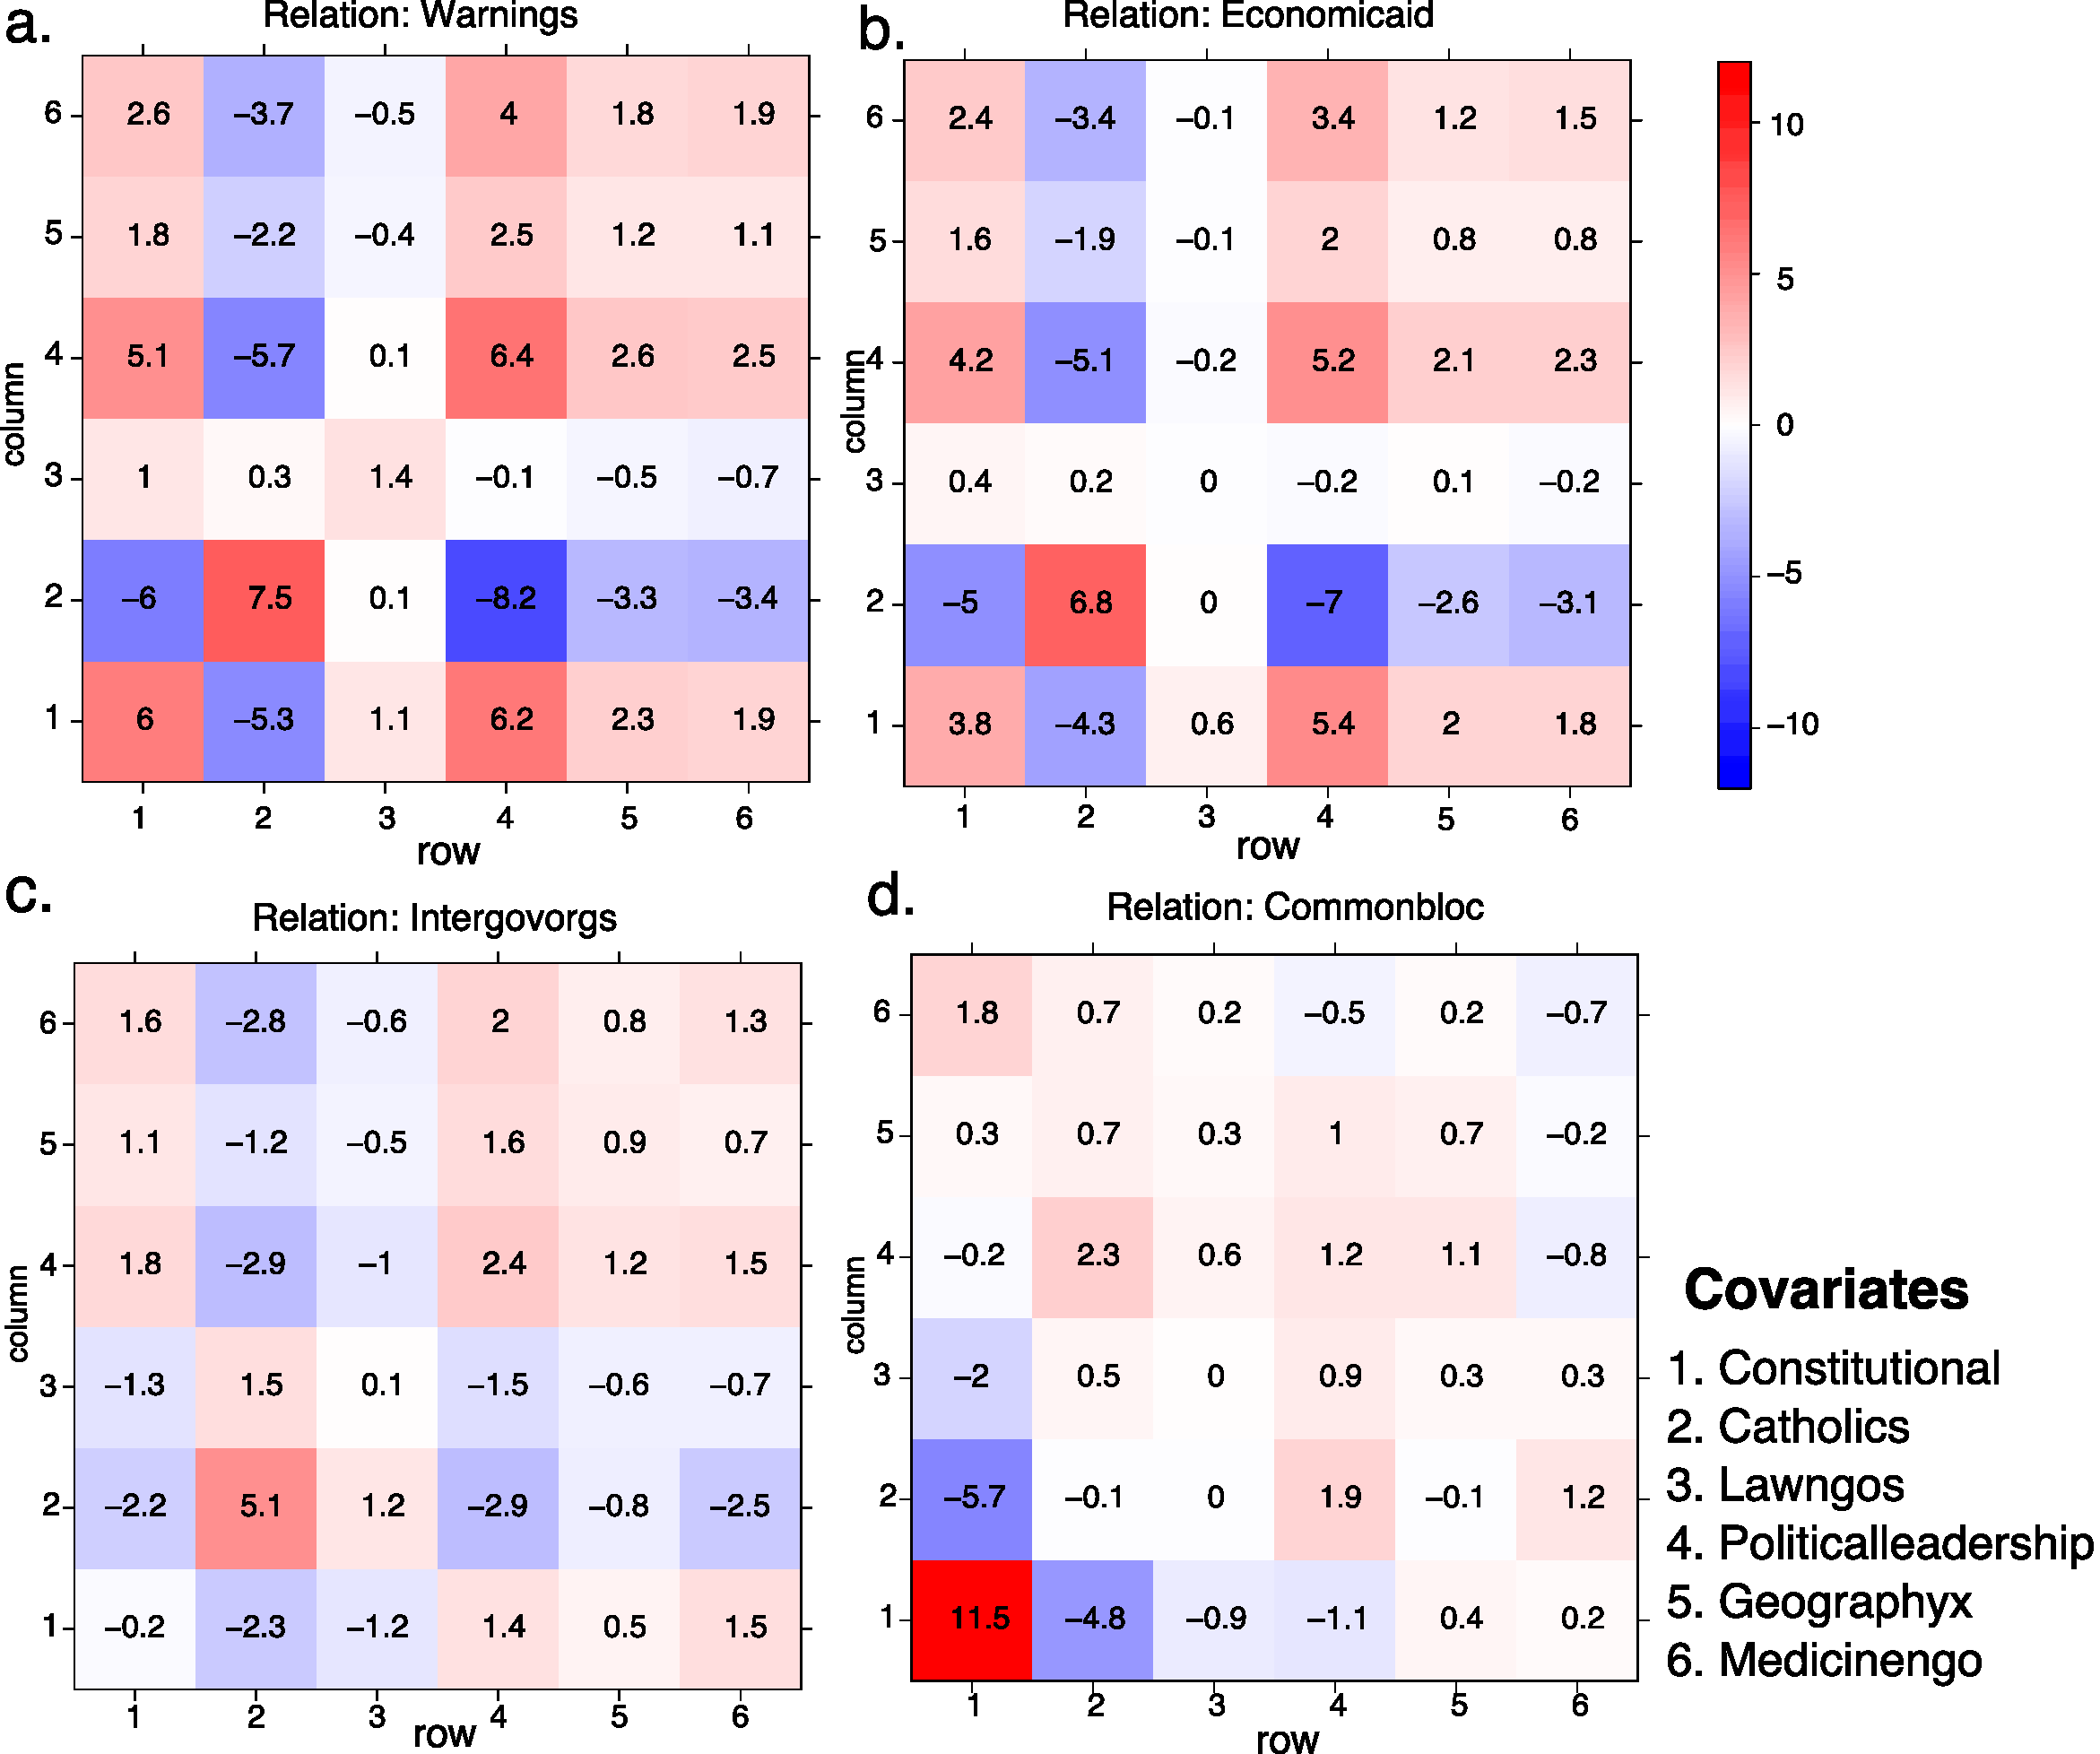
\includegraphics[width=8cm]{coef.pdf}
\caption{Effect estimation in the \emph{Nations} data. Panels (a)-(d) represent the estimated effects of country-level attributes towards the connection probability, for relations \emph{warnning}, \emph{economicaid},\emph{intergovorg}, and \emph{commonblock}, respectively. }\label{fig:est}

\end{figure}


To investigate the effects of dyadic attributes towards connections, we depicted the estimated coefficients $\hat \tB=\entry{\hat b_{ijk}}$ for several relation types (Figure~\ref{fig:est}). Note that entries $\hat b_{ijk}$ can be interpreted as the contribution, at the logit scale, of covariate pair $(i,j)$ ($i$th covariate for the ``sender'' country and $j$th covariate for the ``receiver'' country) towards the connection of relation $k$.  Several interesting findings emerge from the observation. We found that relations belonging to a same cluster tend to have similar covariate effects. For example, the relations \emph{warnings} and \emph{ecnomicaid} are classified into Cluster II, and both exhibit similar covariate pattern (Figure~\ref{fig:est}a-b). Moreover, the majority of the diagonal entries $\hat \tB(i,i,k)$ positively contribute to the connection. This suggests that countries with coherent attributes tend to interact more often than others. We also found that the \emph{constitutional} attribute is an important predictor for the \emph{commonbloc} relation, whereas the effect is weaker for other relations (Figure~\ref{fig:est}d). This is not surprising, as the block partition during Cold War is associated with the \emph{constitutional} attribute. 


\section{Conclusions}

 We have developed a generalized tensor regression with covariates on multiple modes. A fundamental feature of tensor-valued data is the statistical interdependence among entries. Our proposed rank-constrained estimation achieves high accuracy with sound theoretical guarantees. The estimation accuracy is quantified via deviation in the Frobenius norm and K-L divergence. Other measures of accuracy may also be desirable, such as the spectral norm or the infinity norm of the deviation. Exploiting the properties and benefits of different error quantification warrants future research.

\appendix 
\section{Proofs}
\begin{proof}[Proof of Theorem~\ref{thm:main}]
Define $\ell(\tB)=\mathbb{E}(\tL_{\tY}(\tB))$, where the expectation is taken with respect to $\tY\sim \trueB$ under the model with true parameter $\trueB$. We first prove the following two conclusions:
\begin{enumerate}
\item[C1.] There exists two positive constants $C_1$, $C_2>0$, such that, with probability at least $1-\exp(-C_1\log K\sum_k p_k)$, the stochastic deviation, $\tL_{\tY}(\tB)-\ell(\tB)$, satisfies
\[
|\tL_{\tY}(\tB)-\ell(\tB)|=|\langle \tE,\ \tB\times_1\mX_1\times_2\cdots\times_K \mX_K\rangle| \leq C_2\FnormSize{}{\tB} \log K\sqrt{{\prod_k r_k \over \max_k r_k} \sum_k p_k}.
\]
\item[C2.] The inequality $\ell(\hat \tB) - \ell(\trueB) \leq  -{L\over 2}\FnormSize{}{\hat \Theta-\trueT}^2$ holds, where $L>0$ is the lower bound for $\min_{|\theta|\leq \alpha}|b''(\theta)|$. 
\end{enumerate}

To prove C1, we note that the stochastic deviation can be written as:
\begin{align}\label{bound}
\tL_{\tY}(\tB)-\ell(\tB)&=\langle \tY-\mathbb{E}(\tY|\tX),\ \Theta(\tB)\rangle\notag \\
&= \langle \tY- b'(\trueT),\ \Theta\rangle \notag \\
&= \langle \tE\times_1\mX^T_1\times_2\cdots\times_K\mX^T_K,\ \tB\rangle,
\end{align}
where $\tE=\entry{\varepsilon_{i_1,\ldots,i_K}}\stackrel{\text{def}}{=}\tY-b'(\trueT)$. Based on Proposition~\ref{prop}, $\varepsilon_{i_1,\ldots,i_K}$ is sub-Gaussian-$(\phi U)$. Let $\check\tE\stackrel{\text{def}}{=}\tE\times_1\mX^T_1\times_2\cdots\times_K\mX^T_K$. By the property of sub-Gaussian r.v's, $\check \tE$ is a $(p_1,\ldots,p_K)$-dimensional sub-Gaussian tensor with parameter bounded by $C_2=\phi Uc^{K}_2$. Here $c_2>0$ is the upper bound of $\sigma_{\max}(\mX_k)$. Applying Cauchy-Schwarz inequality to~\eqref{bound} yields
\begin{equation}\label{eq:bound2}
|\tL_{\tY}(\tB)-\ell(\tB)|\leq \norm{\check \tE} \nnorm{\tB},
\end{equation}
where $\norm{\cdot}$ denotes the tensor spectral norm and $\nnorm{\cdot}$ denotes the tensor nuclear norm. The nuclear norm $\nnorm{\tB}$ is  bounded by $\nnorm{\tB}\leq \sqrt{{\prod_k r_k \over \max_k r_k}}\FnormSize{}{\tB}$ (c.f.~\cite{wang2018learning,wang2017operator}). The spectral norm $\norm{\check \tE}$ is bounded by $\norm{\check \tE}\leq C_1 Uc^{K} \log K \sqrt{\sum_k p_k}$ with probability at least $1-\exp(-C_2\log K \sum_kp_k)$ (c.f.~\cite{wang2018learning,tomioka2014spectral}). Combining these two bounds with~\eqref{eq:bound2}, we have, with probability at least $1-\exp(-C_2\log K \sum_kp_k)$, 
\[
|\tL_{\tY}(\tB)-\ell(\tB)|\leq C_1Uc_2^{K}\FnormSize{}{\tB} \log K  \sqrt{ {\prod_k r_k\over \max_k r_k}\sum_k p_k}.
\]

Next we prove C2. Applying Taylor expansion to $\ell(\tB)$ around $\trueB$, 
\begin{equation}\label{eq:log}
\ell(\tB)=\ell(\trueB)-{1\over 2}\text{vec}(\tB-\trueB)^T \tH_{\tY}(\check \tB)\text{vec}(\tB-\trueB),
\end{equation}
where $\tH_{\tY}(\check \tB)$ is the (non-random) Hession of ${\partial \ell^2 (\tB)\over\partial^2 \tB}$ evaluated at $\check \tB =\alpha \text{vec}(\alpha \tB+(1-\alpha)\trueB)$ for some $\alpha\in[0,1]$. Recall that $b''(\theta)=\text{Var}(y|\theta)$, because $y\in\mathbb{R}$ follows the exponential family distribution with function $b(\cdot)$. By chain rule and the fact that $\Theta=\Theta(\tB)=\tB\times_1\mX_1\cdots\times_K\mX_K$, the equation~\eqref{eq:log} implies that
\begin{equation}\label{eq:log}
\ell(\tB)-\ell(\trueB)=-{1\over 2}\sum_{i_1,\ldots,i_K}b''(\check \theta_{i_1,\ldots,i_K}) (\theta_{i_1,\ldots,i_K}-\theta_{\text{true},i_1,\ldots,i_K})^2 \leq -{L \over 2}\FnormSize{}{\Theta-\trueT}^2,
\end{equation}
holds for all $\tB\in\tP$, provided that $\min_{|\theta|\leq \alpha}|b''(\theta)|\geq L>0$. In particular, the inequality~\eqref{eq:log} also applies to the constrained MLE $\hat \tB$. So we have
\begin{equation}\label{upperbound}
\ell(\hat \tB)-\ell(\trueB)\leq -{L \over 2}\FnormSize{}{\hat \Theta-\trueT}^2.
\end{equation}
Now we have proved both C1 and C2. Note that $\tL_{\tY}(\hat \tB)- \tL_{\tY}(\trueB)\geq 0$ by the definition of $\hat \tB$, This implies that
\begin{align}
0&\leq \tL_{\tY}(\hat \tB)- \tL_{\tY}(\trueB) \\
&\leq \left(\tL_{\tY}(\hat \tB)-\ell(\hat \tB)\right)-\left( \tL_{\tY}(\trueB)-\ell(\trueB)\right)+\left(\ell(\hat \tB)-\ell(\trueB)\right)\\
&\leq \langle\tE,\ \Theta-\trueT    \rangle -{L\over 2}\FnormSize{}{\hat \Theta-\trueT}^2,
%&\leq 2\sup_{\tB}|\tL_{\tY}(\tB)-\ell(\tB)|-{L\over 2}\FnormSize{}{\hat \Theta-\trueT}^2
\end{align}
where the second line follows from~\eqref{upperbound}. Therefore,
\begin{align}\label{eq:1}
\FnormSize{}{\hat \Theta-\trueT}&\leq {2\over L}\big\langle \tE,\ {\hat \Theta -\trueT \over \FnormSize{}{\hat \Theta-\trueT}} \big\rangle\notag \\
&\leq {2\over L}\sup_{\Theta: \FnormSize{}{\Theta}=1, \Theta=\tB\times_1\mX_1\times_2\cdots\times_K \mX_K}\langle \tE,\ \Theta \rangle\notag \\
&\leq {2\over L}\sup_{\tB\in\tP: \FnormSize{}{\tB}\leq \prod_k \sigma^{-1}_{\min}(\mX_k)} \langle \tE,\ \ \tB\times_1\mX_1\times_2\cdots\times_K\mX_K\rangle.
\end{align}
Combining~\eqref{eq:1} with C1 yields the desired conclusion. 

%\[
%\FnormSize{}{\hat \Theta-\trueT}\leq {2R\over L}  \sum_{i=1} p_i ()
%\]
%\[
%\FnormSize{}{\hat \Theta-\trueT}^2\leq {2\over L}\sup_{\tB: \FnormSize{}{\tB}=1}|\tL_{\tY}(\tB)-\ell(\tB)|\leq {2\over L} \sum_k p_k
%\]
%holds with probability at least $1-\exp(C_1\sum_k p_k)$.
\end{proof}

\begin{prop}[sub-Gaussian residual]\label{prop}
Define the residual tensor $\tE=\entry{\varepsilon_{i_1,\ldots,i_K}}=\tY-b'(\Theta)\in\mathbb{R}^{d_1\times \cdots \times d_K}$. Under the Assumption A2, $\varepsilon_{i_1,\ldots,i_K}$ is a sub-Gaussian random variable with sub-Gaussian parameter bounded by $\phi U$, for all $(i_1,\ldots,i_K)\in[d_1]\times\cdots\times[d_K]$.
\end{prop}
\begin{proof} The proof is similar to Lemma 3 in~\cite{fan2019generalized}. For ease of presentation, we drop the subscript $(i_1,\ldots,i_K)$ and simply write $\varepsilon$ ($=y-b'(\theta)$). For any given $t\in\mathbb{R}$, we have
\begin{align}
\mathbb{E}(\exp(t\varepsilon|\theta)&=\int c(x) \exp\left({\theta x - b(\theta)\over \phi}   \right)\exp \left(t(x-b'(\theta))\right)dx\\
&=\int c(x)\exp \left( {(\theta + \phi t)x - b (\theta+\phi t)+b(\theta+\phi t)-b(\theta)-\phi t b'(\theta) \over \phi}\right)dx\\
&=\exp\left( {b(\theta+\phi t)-b(\theta)-\phi t b'(\theta) \over \phi} \right)\\
&\leq \exp\left(\phi U t^2\over 2 \right),
\end{align}
where $c(\cdot)$ and $b(\cdot)$ are known functions in the exponential family corresponding to $y$. 
Therefore, $\varepsilon$ is sub-Gaussian-$(\phi U)$. 
\end{proof}

\begin{proof}[Proof of Theorem~\ref{thm:KL}]
The proof is similar to~\cite{baldin2018optimal}. We sketch the main steps here for completeness. Recall that $\ell(\tB)=\mathbb{E}(\tL_{\tY}(\tB))$. By the definition of KL divergence, we have that,
\begin{align}
\ell(\hat \tB)&=\ell(\trueB)-\sum_{(i_1,\ldots,i_K)} KL(\theta_{\text{true}, i_1,\ldots, i_K}, \hat \theta_{i_1,\ldots,i_K})\\
&=\ell(\trueB)-\text{KL}(\mathbb{P}_{\tY_{\text{true}}},\ \mathbb{P}_{\hat \tY}),
\end{align}
where $\mathbb{P}_{\tY_{\text{true}}}$ denotes the distribution of $\tY|\tX$ with true parameter $\trueB$, and $\mathbb{P}_{\hat \tY}$ denotes the distribution with estimated parameter $\hat \tB$. Therefore
\begin{align}
\text{KL}(\mathbb{P}_{\tY_{\text{true}}},\ \mathbb{P}_{\hat \tY}) &= \ell(\trueB)-\ell(\hat \tB)\\
&={1\over 2}\sum_{i_1\ldots,i_K}b''(\check \theta_{i_1,\ldots,i_K})(\theta_{i_1,\ldots,i_K}-\theta_{\text{true},i_1,\ldots,i_K})^2\\
&\leq {U\over 2} \FnormSize{}{\Theta-\trueT}^2\\
&\leq {U \over 2}c^{2K}_2\FnormSize{}{\tB-\trueB}^2,
\end{align}
where the second line comes from~\eqref{eq:log}, and $c_2>0$ is the upper bound for the $\sigma_{\max}(\mX_k)$. The result then follows from Theorem~\ref{thm:main}.
\end{proof}

\section{Time complexity}
The computational complexity of our tensor regression model is $O(d^3+d)$ for each loop of iterations, where $d=\prod_k d_k$ is the total size of the response tensor. More precisely, the update of core tensor costs $O(r^3d^3)$, where $r=\sum_k r_k$ is the total size of the core tensor. The update of factor matrix $\mM_k$ involves solving $p_k$ separate GLMs. Solving those GLMs requires $O(r_k^3 p_k + p_kr_k^3 dd^{-1}_k)$, and therefore the cost for updating $K$ factors in total is $O( \sum_k r^3_k p_k d_k + d\sum_k r_k^3 p_k d_k^{-1})\approx O(\sum p_k d_k +d)\approx O(d)$. 
\section{Additional results for real data analysis}
Here we provide additional results for the real data analysis. 


\subsection{HCP data analysis}

The Supplement Figur~\ref{fig:s1} compares the estimated coefficients from our method (tensor regression) with those from classical GLM approach. A classical GLM is to regress the brain edges, one at a time, on the individual-level covariates, and this logistic model is repeatedly fitted for every edge $\in [68]\times [68]$. As we can see in the figure, our tensor regression shrinkages the coefficients towards center, thereby enforcing the sharing between coefficient entries. 

\begin{figure}[t]
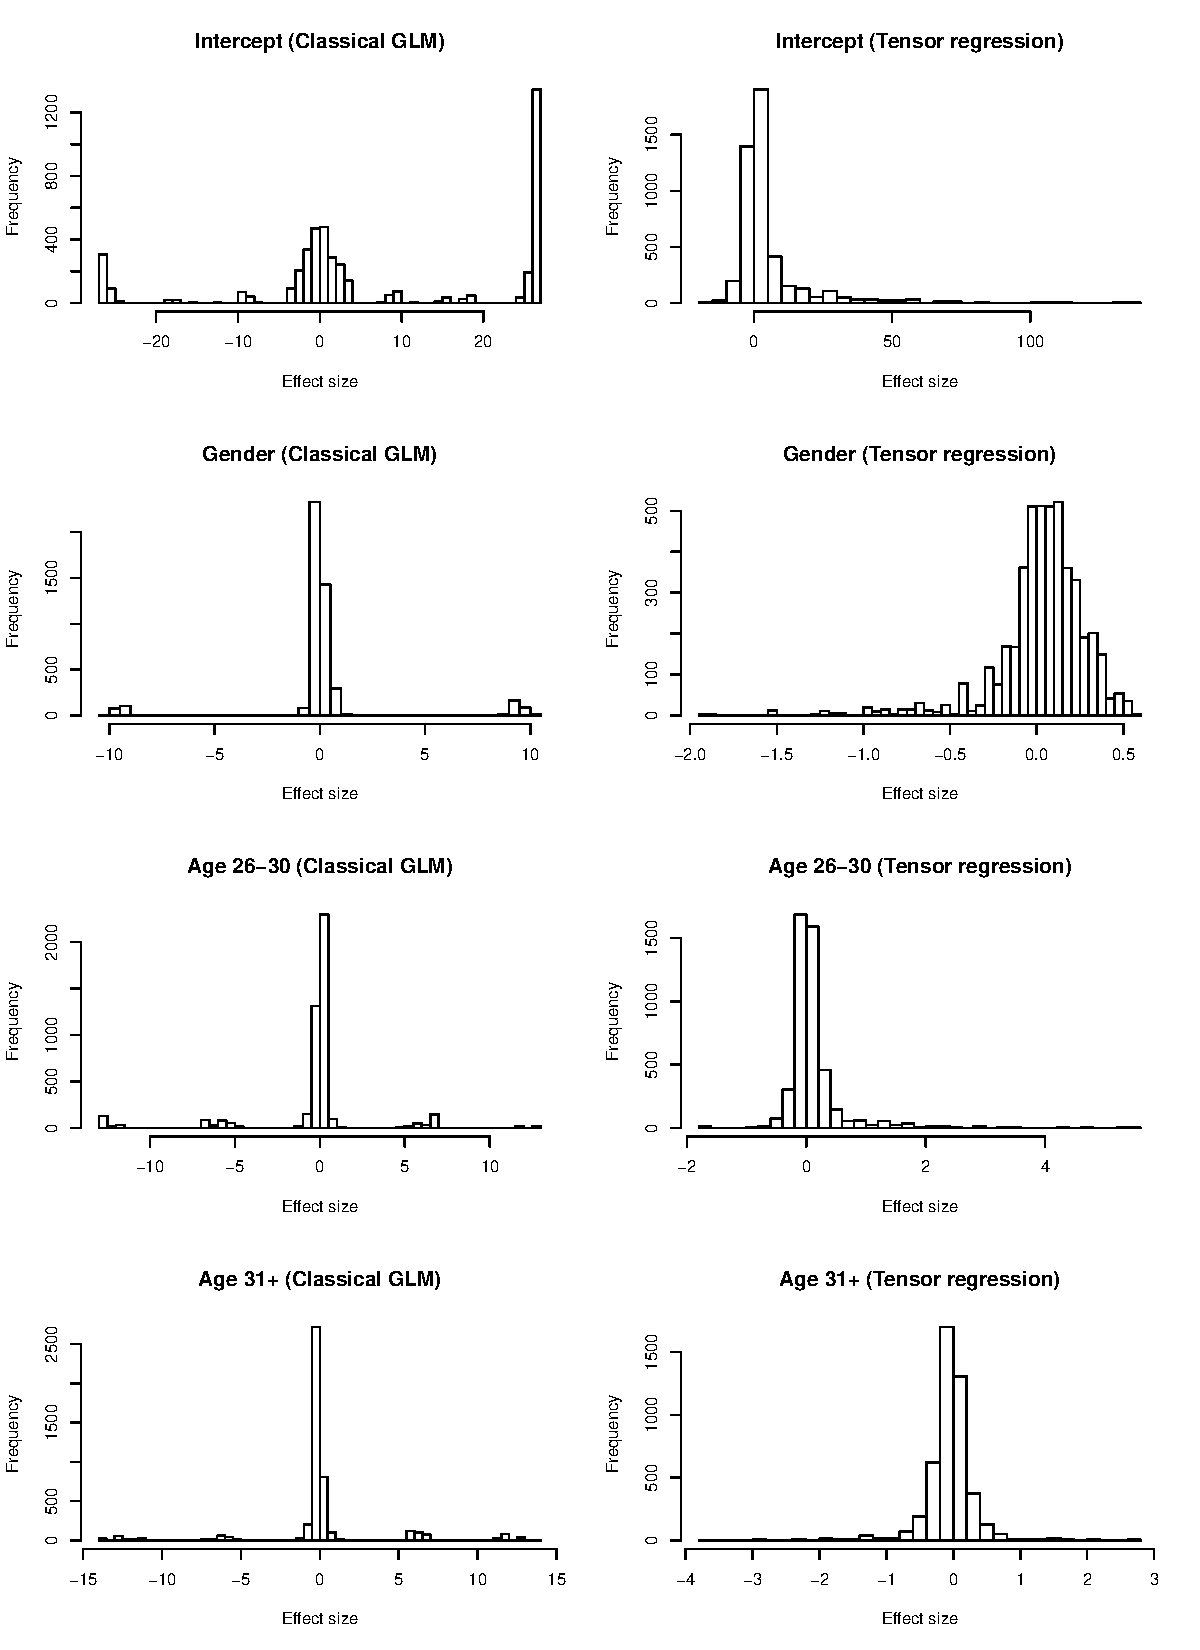
\includegraphics[width=17cm]{compare.pdf}
\caption{Comparison of coefficient estimation in the HCP data.}\label{fig:s1}
\end{figure}

\subsection{Nations data analysis}
Supplement table~\ref{tab:s1} summarizes the $K$-means clustering of the 56 relations based on the $3^{\text{rd}}$ mode factor $\mM_3\in\mathbb{R}^{56\times 4}$ in the tensor regression model. 

\begin{table}[H]
\begin{tabular}{c|l}
\hline
\multirow{4}{*}{Cluster I}  &officialvisits, intergovorgs,  militaryactions, violentactions, duration, \\
&negativebehavior, boycottembargo, aidenemy, negativecomm, accusation, \\
& protestsunoffialacts,    nonviolentbehavior, emigrants, relexports,   \\
& timesincewar, commonbloc2, rintergovorgs3, relintergovorgs\\
\hline
\multirow{4}{*}{Cluster II}& economicaid, booktranslations, tourism, relbooktranslations, releconomicaid, \\
& conferences, severdiplomatic, expeldiplomats, attackembassy, unweightedunvote,\\
& reltourism, tourism3, relemigrants, emigrants3, students, relstudents, \\
&exports, exports3, lostterritory, dependent, militaryalliance, warning  \\
\hline
\multirow{2}{*}{Cluster III} & treaties, reltreaties, exportbooks, relexportbooks, weightedunvote, ngo, \\
&relngo, ngoorgs3, embassy, reldiplomacy, timesinceally, independence, commonbloc1\\
\hline
Cluster IV & commonbloc0, blockpositionindex\\
\end{tabular}
\caption{$K$-means clustering of relations based on factor matrix in the coefficient tensor.}\label{tab:s1}
\end{table}



\section*{Acknowledgements}
This research was supported by NSF grant DMS-1915978 and the University of Wisconsin-Madison, Office of the Vice Chancellor for Research and Graduate Education with funding from the Wisconsin Alumni Research Foundation. 

\bibliographystyle{unsrt}
\bibliography{tensor_wang}

\end{document}